
\section{Architecture Integration}

\subsection{Model Support}

\begin{table}[H]
\centering
\small
\begin{tabular}{llllll}
\toprule
\textbf{Model} & \textbf{Attention class} & \textbf{Nested?} & \textbf{RoPE?} & \textbf{GQA?} & \textbf{Verified} \\
\midrule
DistilBERT & \texttt{MultiHeadSelfAttention} & No & No & No &  \\
RoBERTa & \texttt{BertSelfAttention} (nested) & Yes & No & No &  \\
GPT-2 & \texttt{GPT2Attention} (Conv1D) & No & No & No &  \\
Qwen3.5 & \texttt{Qwen3Attention} & No & Yes & Yes & 0.85 \\
\bottomrule
\end{tabular}
\end{table}

\subsection{Adaptive Rank}

\begin{lstlisting}
num\_layers = config.num\_hidden\_layers
if num\_layers \textgreater{} 12:
    self.rank = max(self.rank, 128)
elif num\_layers \textgreater{} 6:
    self.rank = max(self.rank, 64)
self.rank = max(1, min(self.rank, self.head\_dim))
\end{lstlisting}

The rank is capped at \texttt{head\_dim} because projecting beyond the head 
dimension is not a compression.

\subsection{Weight Extraction}

\subsubsection{DistilBERT}

\begin{lstlisting}
extracted["q"] = src.q\_lin.weight
extracted["k"] = src.k\_lin.weight
extracted["v"] = src.v\_lin.weight
extracted["o"] = src.out\_lin.weight
\end{lstlisting}

\subsubsection{RoBERTa (nested)}

\begin{lstlisting}
s = src.self
extracted["q"] = s.query.weight
extracted["k"] = s.key.weight
extracted["v"] = s.value.weight
extracted["o"] = src.output.dense.weight
\end{lstlisting}

\subsubsection{GPT-2 (Conv1D)}

\begin{lstlisting}
w = src.c\_attn.weight.t()
q\_w, k\_w, v\_w = w.chunk(3, dim=0)
extracted["q"] = q\_w
extracted["k"] = k\_w
extracted["v"] = v\_w
extracted["o"] = src.c\_proj.weight.t()
\end{lstlisting}

\subsection{Random Projection Buffer}

\begin{lstlisting}
self.register\_buffer(
    "proj",
    torch.randn(self.num\_heads, self.head\_dim, self.rank) * (self.head\_dim ** -0.5)
)
\end{lstlisting}

\textbf{Key insight.} Buffers are:
\begin{itemize}
\item Not counted in \texttt{numel()} of \texttt{parameters()}.
\item Saved with the model (state\_dict).
\item Not updated by optimizers.

\end{itemize}
\subsection{Nested Encoder Handling}

For RoBERTa/BERT, \texttt{is\_nested\_encoder = True} means RPC returns the raw 
context without applying its own \texttt{out\_proj}. The outer \texttt{attention.output.dense} 
applies the actual output projection.

\begin{lstlisting}
if self.is\_nested\_encoder:
    out = context
else:
    out = self.out\_proj(context)
\end{lstlisting}

\subsection{Injection}

\begin{lstlisting}
def inject\_rpc(layer, model\_config=None, old\_attn=None, **kwargs):
    src = old\_attn or find\_attention(layer)
    new\_attn = RPCAttention(config=model\_config, pretrained\_attn=src, **kwargs)
    replace\_attention(layer, new\_attn)
    return new\_attn
\end{lstlisting}

\subsection{Failure Modes}

\begin{table}[H]
\centering
\small
\begin{tabular}{lll}
\toprule
\textbf{Failure} & \textbf{Detection} & \textbf{Response} \\
\midrule
Missing projection & \texttt{copy\_weights} raises & Injection fails \\
Small Frobenius norm & Explicit check & Raises RuntimeError \\
Nested encoder mis-set & Logits differ & Manual fix \\
OOM & RuntimeError & Reduce batch \\
\bottomrule
\end{tabular}
\end{table}

\textbf{Critical.} RPC's \texttt{copy\_weights} uses \texttt{raise RuntimeError}, and 
\texttt{inject\_rpc} also raises:

\begin{lstlisting}
except Exception as e:
    logger.error("inject\_rpc failed: \%s", e)
    raise RuntimeError(f"Injection failed")
\end{lstlisting}

This is \textbf{stricter} than NHA/EAT but similar to ASVD and OHA.

\subsection{Registry}

\begin{lstlisting}
@ATTENTION\_REGISTRY.register("rpc")
@ATTENTION\_REGISTRY.register("rpc\_attention")
class RPCAttention(BaseAttention):
    ...
\end{lstlisting}

\subsection{Causality}

\textbf{Verification.} Gradient of output at position $i$ w.r.t. input at 
position $j > i$ is zero.

\subsection{Cross-Attention}

RPC's forward accepts \texttt{encoder\_hidden\_states} as an argument but does not 
use it. Cross-attention is effectively unsupported.
\begin{lstlisting}

---
\end{lstlisting}

\begin{figure}[H]
\centering
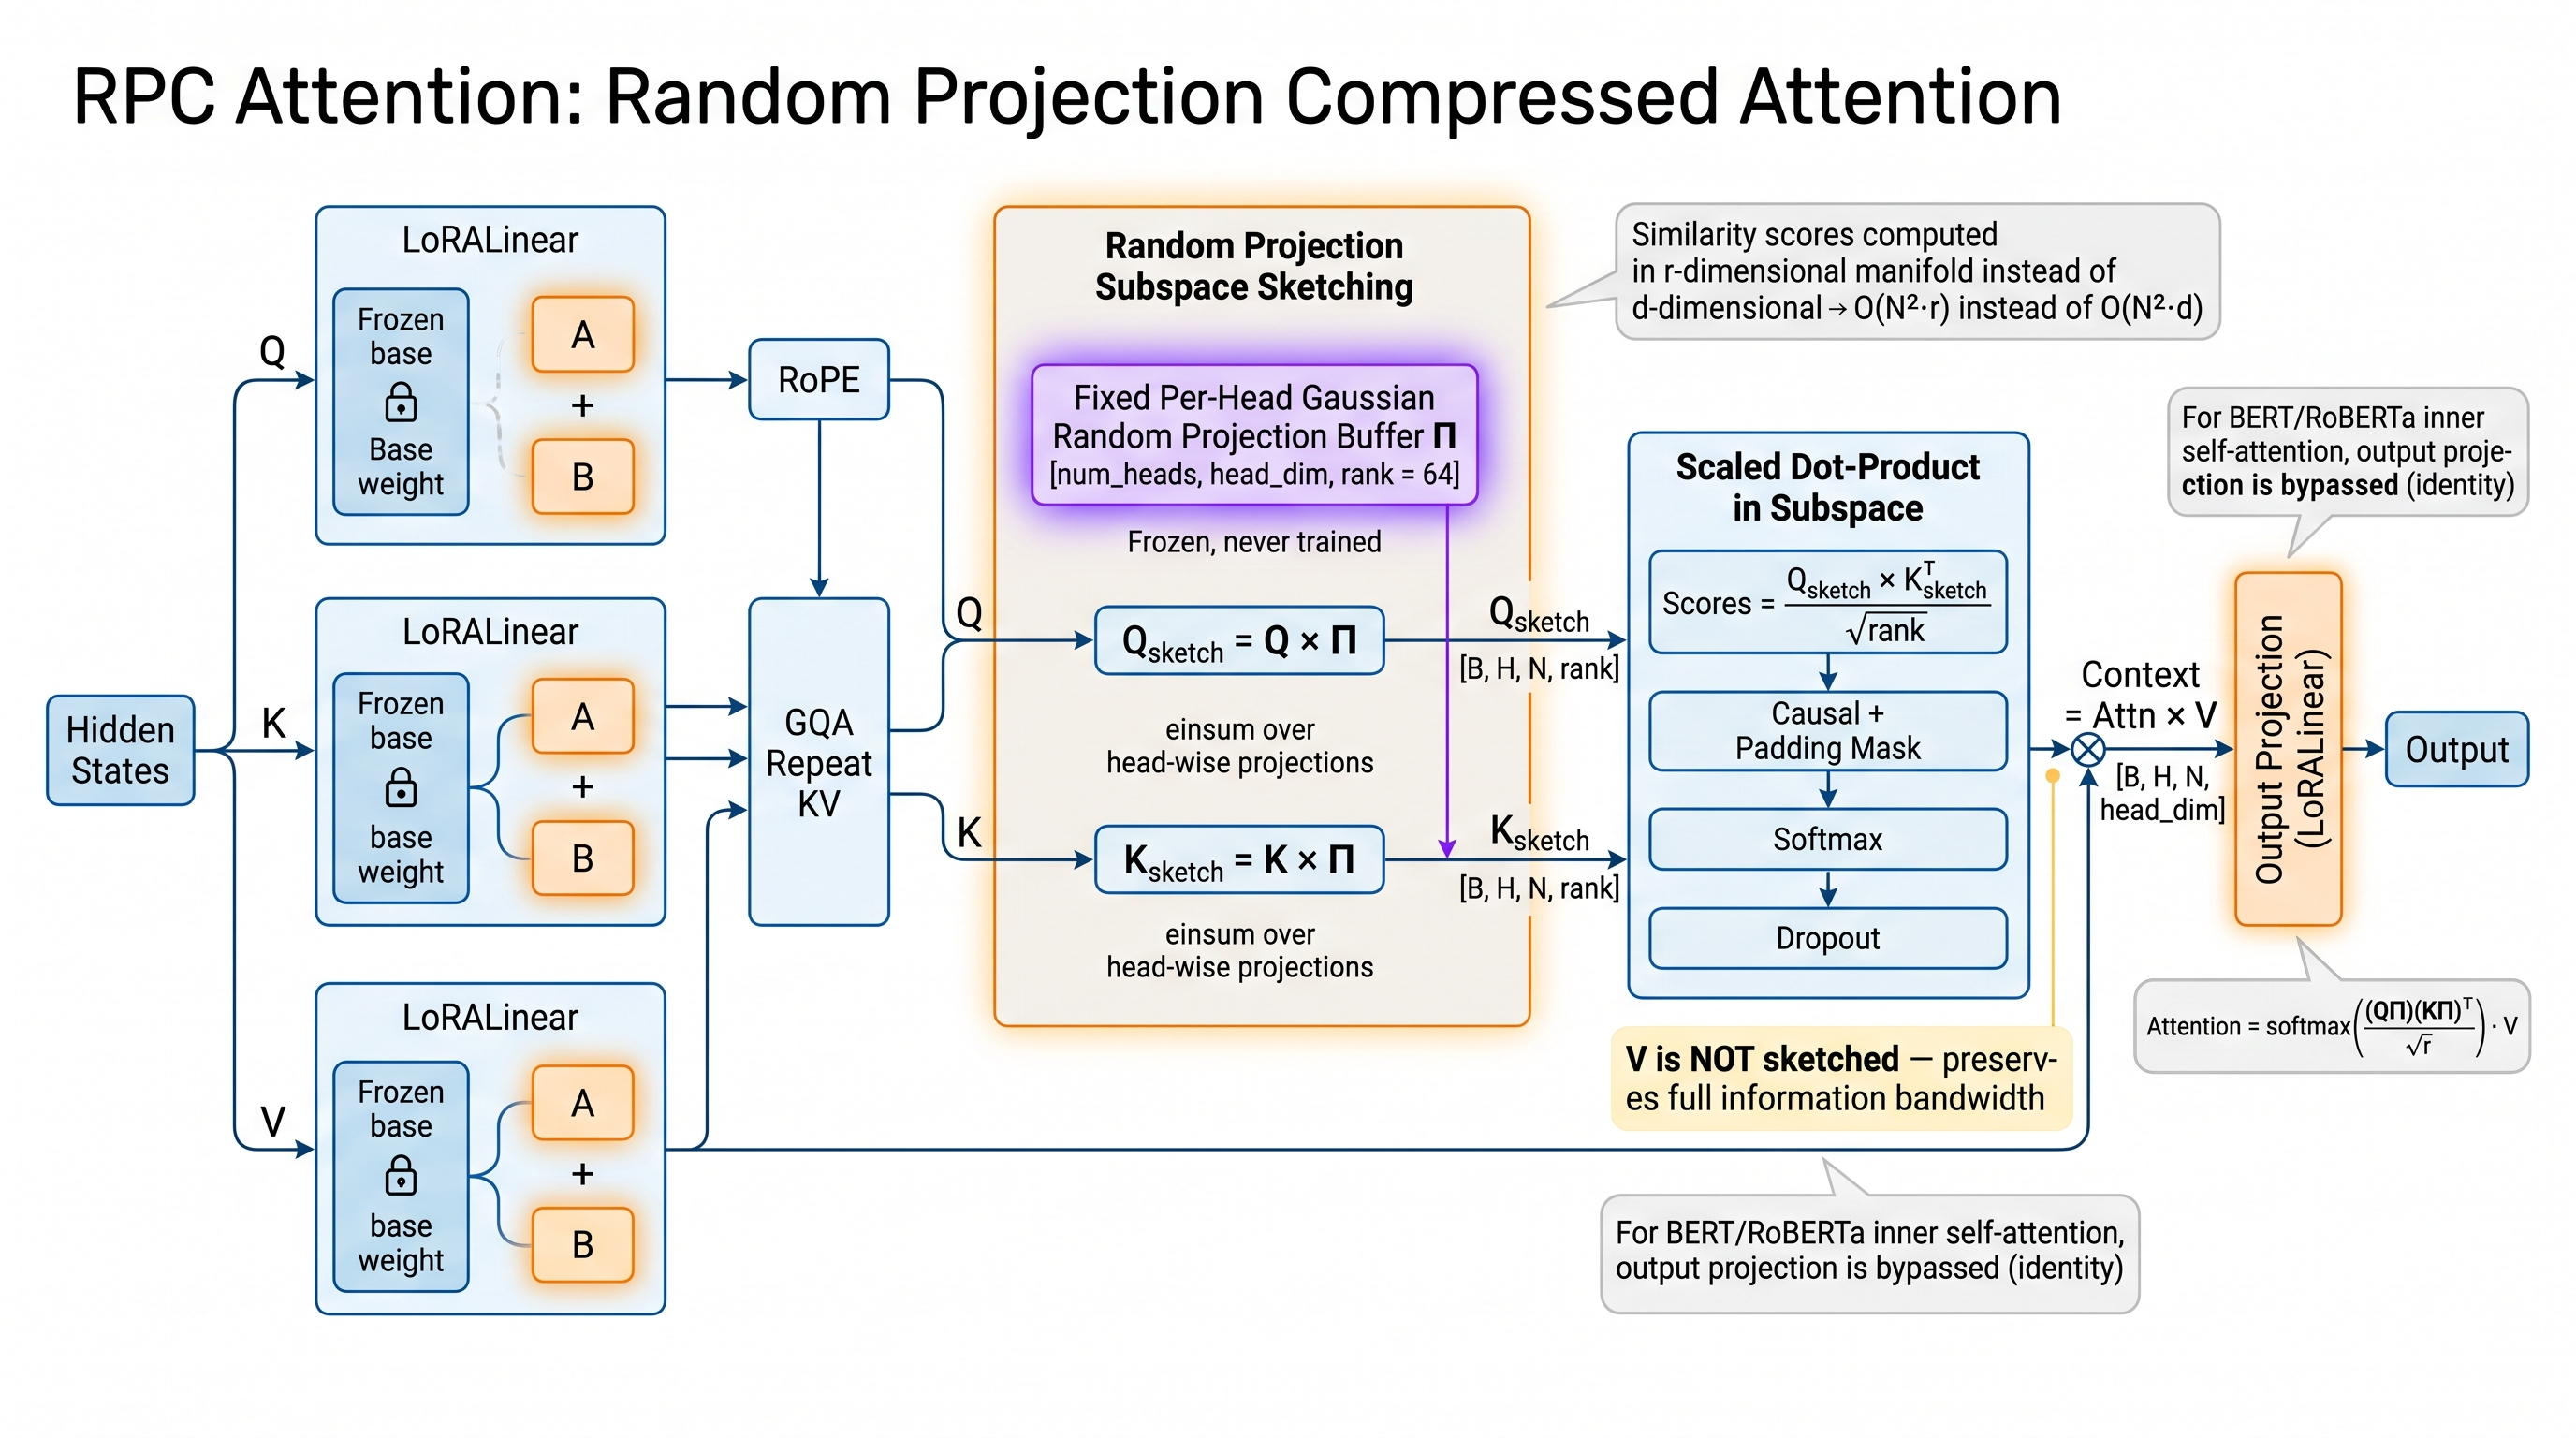
\includegraphics[width=\linewidth]{figures/architecture.jpeg}
\caption{High-level architectural diagram of rpc.}
\label{fig:arch\_rpc}
\end{figure}

